\label{sect:nucleus}


Examining the {\em Spitzer}-IRS spectral data cube for the nuclear region, we noticed that different spectral features vary spatially within this region.
The 11.2~$\mu$m PAH emission is discrete and patchy (Figure \ref{nuc11}a).  
Indeed, the majority of the 11.2~$\mu$m  PAH emission is from a region 15\arcsec\ north of the nucleus (00:42:43.947, +41:16:22.92) and not from 
the nucleus itself. Weaker 11.2~$\mu$m PAH emission is also found near the edge of the map peaking at 00:42:45.497, +41:15:43.97 and near 00:42:45.869; +41:16:11.38.
The locations of the two weaker 11.2~$\mu$m PAH emission peaks are also near positions exhibiting CO(2-1) line emission \citep[\#36 and 28 of][the strongest 11.2~$\mu$m PAH emission peak is outside the CO FOV]{Melchior2013}. 
On the other hand, the centre shows no PAH emission, but it does have silicate emission around 9.7~$\mu$m, which comes only from the nucleus and is not present in the North region (Figure \ref{nuc11}b).%
\footnote{The spatial resolution and pixel scale of the ISOCAM data are not sufficient to resolve the centre  and north regions.}
Although [NeIII] 15.5~$\mu$m line emission is strong at the three locations with 11.2~$\mu$m PAH emission and weak(er) at the nucleus, 
it is also present across the nuclear region and thus distinct from that of the silicate and PAH emission. 

Some structures  seen in the optical near the M31 nucleus, such as the double nucleus and cluster of young stars, cannot be resolved with the data discussed here.
The IRS spectral cubes have pixel sizes of 1\farcs8, and the SL PSF FWHM is 2.5--3\arcsec depending on the wavelength,
while the two components of the nucleus are separated by only 0\farcs5 \citep{Bender2005}.
However, the nuclear silicate emission and the north 11.2~$\mu$m  PAH emission appear to be 
marginally spatially resolved: 
their radial profiles have full widths at half maximum (FWHM) of 5--7\arcsec\ (corresponding to 19--27pc).
To examine the two regions in more detail, 
we extracted spectra from the centre and the North regions using  $9\arcsec \times 9\arcsec$ 
square apertures as shown in Figures~\ref{fig:nuc_pahfit}, ~\ref{fig:nuc_silicates} and~\ref{smithspec}. 
Both spectra show a blue continuum and atomic fine-structure lines but they exhibit distinct dust emission consistent with the spatial maps: PAH emission is detected in the north spectrum while silicate emission is seen towards the nucleus. 

\begin{figure}
\centering
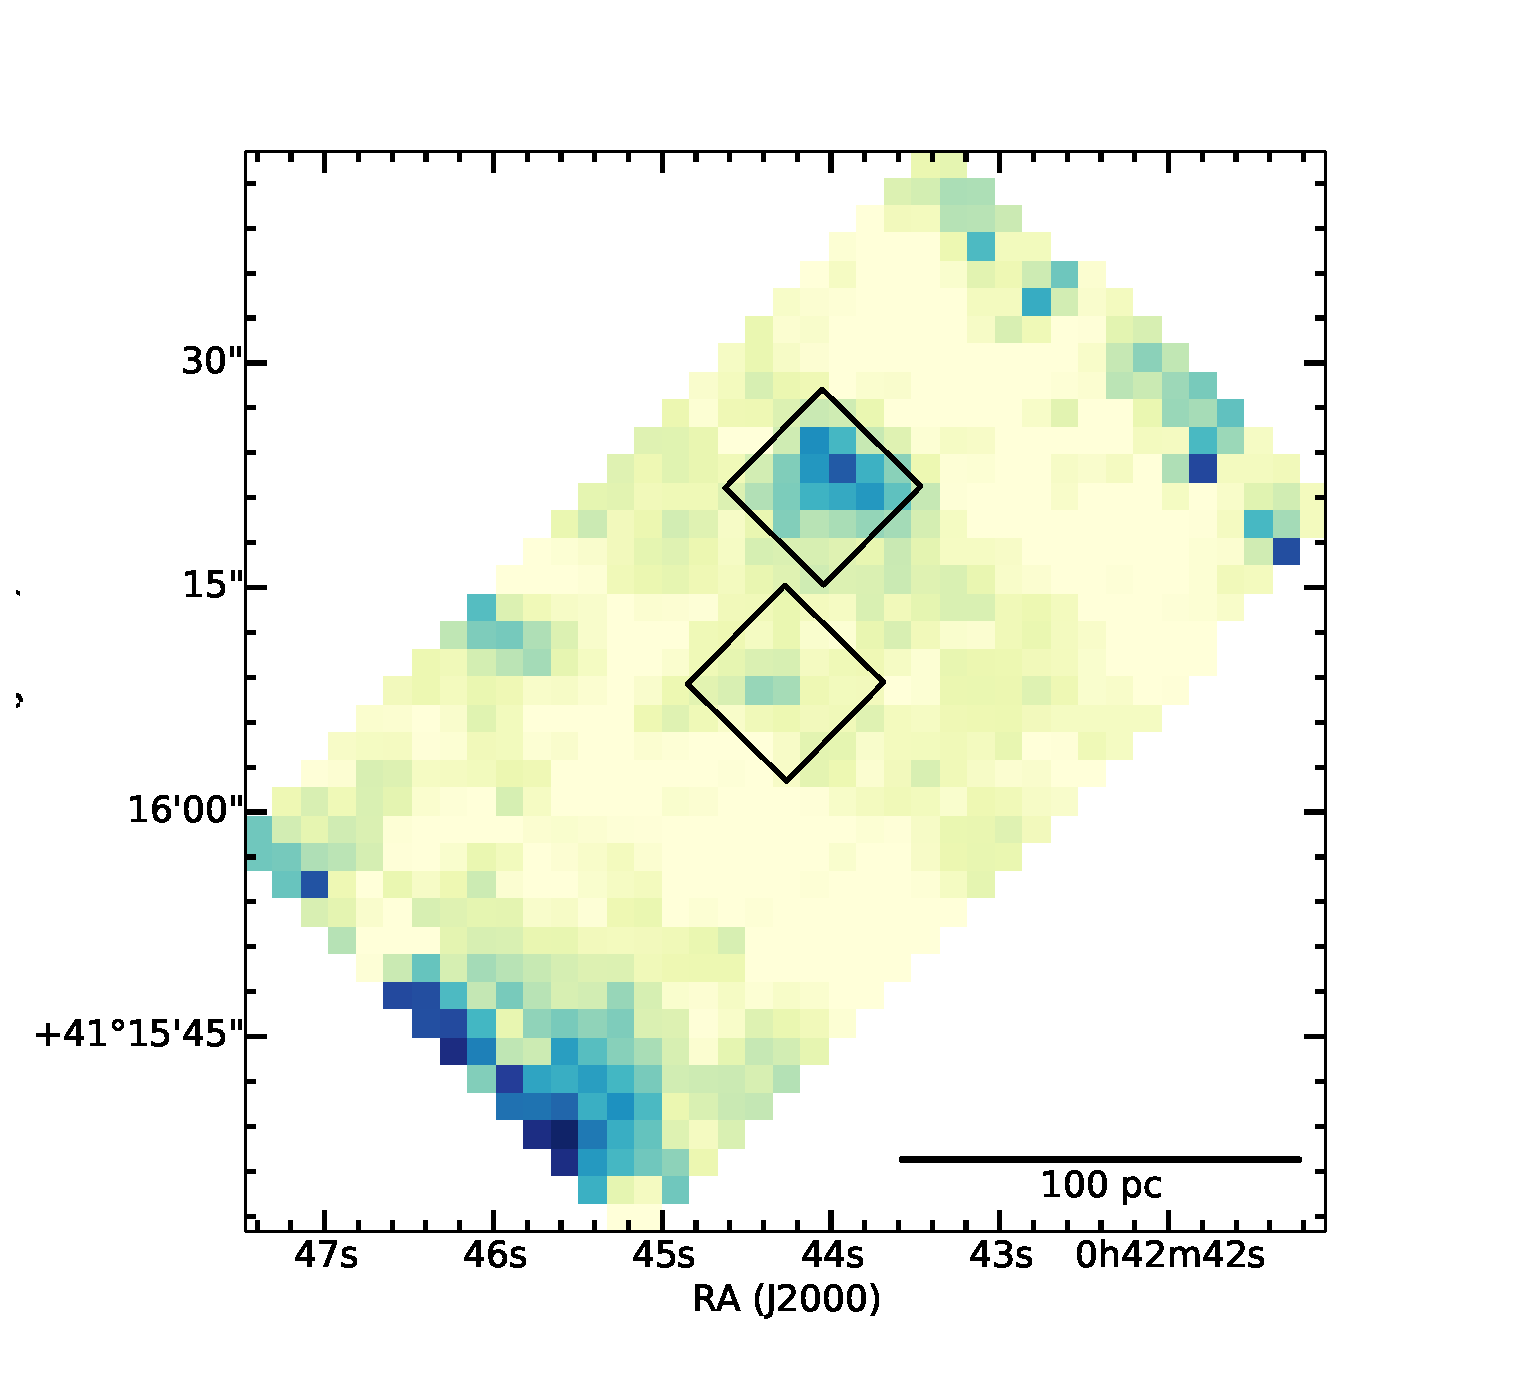
\includegraphics[scale = 0.25]{./fig10a.eps}
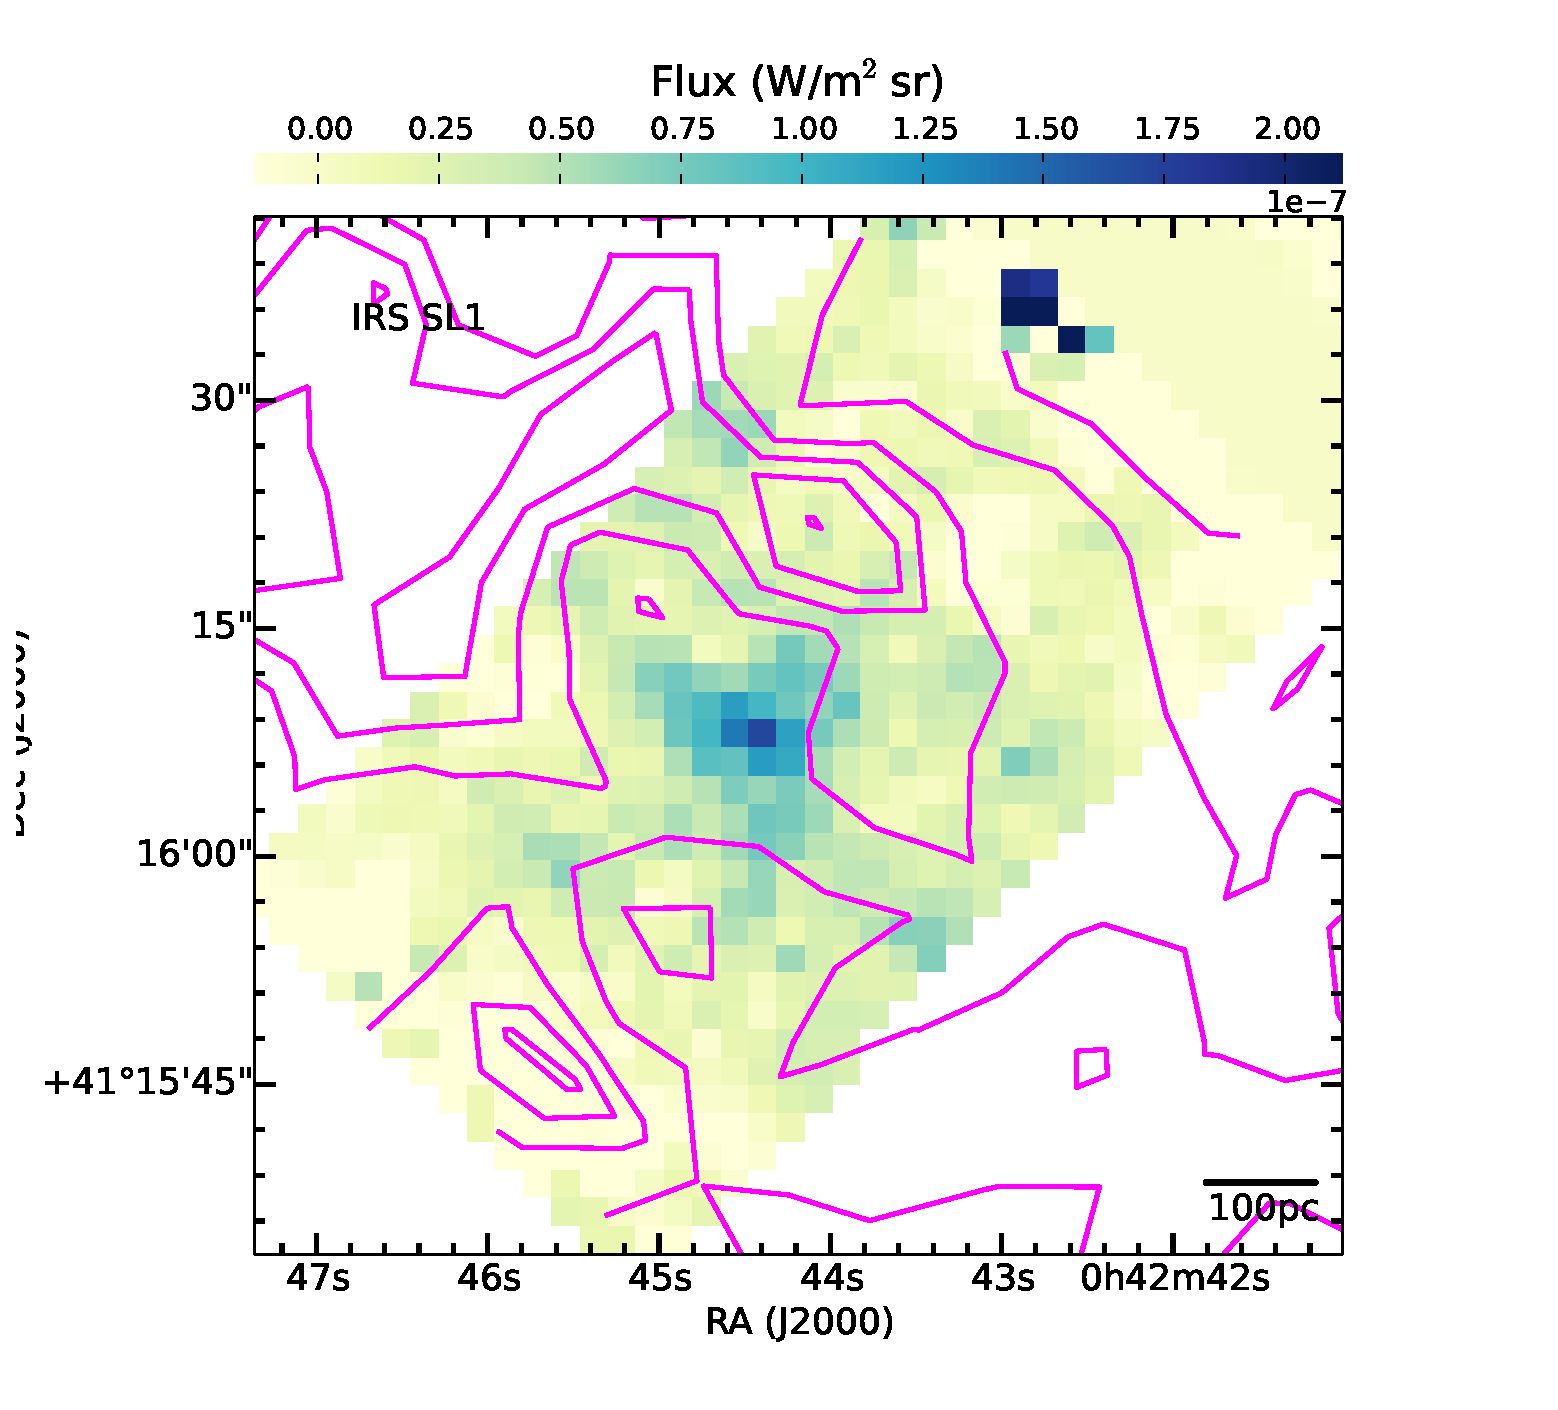
\includegraphics[scale = 0.25]{./fig10b.eps}
\caption{
Integrated strength of the 11.2~$\mu$m PAH emission (top panel) and the silicate emission (from 9 to 11~$\mu$m, continuum subtracted; bottom panel) 
around the nucleus of M31. 
The  two black boxes in the top panel are the 15\arcsec\ $\times$ 15\arcsec\ sub-apertures (centre and north region) used to extract spectra.  
The small white circle in the bottom panel shows a position halfway between the two components of the nucleus; these
components are separated by 0\farcs5, which is well below the IRS spatial resolution. The contours in the bottom panel indicate
the distribution of 3.6~$\mu$m luminosity in the same region, indicating the orientation of the M31 bulge.
}
\label{nuc11}
\end{figure}


Figure~\ref{fig:nuc_pahfit} (top) shows the results of PAHFIT applied to the spectrum of the north region. Atomic fine-structure lines of Ne and S are detected as well as H$_2$ emission at 17~$\mu$m. In addition, PAH emission is clearly detected at 11.3~$\mu$m and at 15-20~$\mu$m while it is weak or absent at 6--8~$\mu$m. We compared the PAH emission with that of the HII-type galaxy NGC0337 in Figure~\ref{fig:nuc_pahfit} (bottom). Despite the enhanced noise level at the shorter wavelengths, it is clear that the emission shortwards of 10 $\mu$m is atypical for PAHs but rather seem to exhibit a broad plateau from $\sim$6 to $\sim$7.5 $\mu$m. Indeed, 6.2~$\mu$m  PAH emission may be hidden in this broad plateau but the typical 7.7 and 8.6~$\mu$m are absent resulting in a decrease of the 7.7/11.2 ratio by roughly a factor of 10 compared to that of NGC0337. This is consistent with the atypical PAH emission in some low-luminosity active galactic nuclei (LLAGN) reported by \citet{Smith:2007lr}.

%REF
%The main problem that I have with the current discussion in S4.4 is, fundamentally, the fact that there is no interpretation of the strong continuum rising to the blue that dominates the spectra. Is this a stellar continuum or an AGN-torus like emission? The IRAC 1 and 2 plus 2MASS data will tell.
%
%I strongly suspect these are stars and this provides a much simpler explanation of the weak 8 um features. Similar strong 11.2 bands are seen in elliptical galaxies with abundant old star populations (e.g. Kaneda et al 2008). Bregman et al 2008 have shown that this apparent weakness of the 8 um emission is induced by the particular shape of the underlying continuum.
%
%In order to assess this possibility it is essential to study the shape of the SED to shorter wavelengths (IRAC 1 and 2 and 2MASS) those data will allow to distinguish readily between stellar continuum and AGN-torus emission.
%
%In fact the region that you isolate as being peculiar is probably not so. I attach a figure which I made using the IRAC 2 and IRAC 4 images from the Spitzer Heritage Archive. I have convolved the IRAC 2 image using Karl Gordon's kernels. After that I have played with the scaling to best subtract the IRAC 2 from the IRAC 4. In this way I automatically correct for any average features in the ``continuum''. In the example I send, I have probably over-subtracted a little. What is striking in the residual image is 8 um emission in excess of the continuum exactly where you detect your 11.2 PAH band.


The central spectrum exhibit silicate emission, blue continuum emission and fine-structure line emission of [NeII] at 12.8$\mu$m, [NeIII] at 15.5$\mu$m and [SIII] at 18.7$\mu$m (Figure~\ref{fig:nuc_silicates}, top). We adapted PAHFIT so that it includes Gaussian profiles to represent the silicate emission and used this modified PAHFIT to fit the continuum emission of both star light and dust towards the nucleus (Figure~\ref{fig:nuc_silicates}, top). While the silicate emission is not well fitted due to its asymmetry, the underlying continuum is well represented by the PAHFIT results. To characterize the silicate emission profile, we compared the continuum-subtracted silicate profile with the silicate absorption profile of the Galactic centre \citep{Chiar2006} as well as the silicate emission profile observed towards the type 1 (i.e., face-on) LINER nucleus of M81 \citep[][Figure~\ref{fig:nuc_silicates}, bottom]{Smith2010}. For the latter, we adopted a spline continuum anchored at 8.36, 8.83, 24.7, 26.45, and 27.79 $\mu$m (Figure~\ref{fig:nuc_silicates}, middle). Compared to the silicate absorption profile towards the Galactic centre, the M31 silicate emission is clearly displaced towards longer wavelengths and the red wing is slightly less steep resulting in a slightly broader profile. This is consistent with previous results reporting that the silicate emission towards  the M81 nucleus as well as towards several galaxies is redshifted and broader than the silicate absorption seen towards galactic sources \citep[e.g.][]{Sturm2005, Sturm2006, Netzer2007, Smith2010}. Contrasting the spectral properties of the nuclei of M31 and M81, we find that the ``9.7"~$\mu$m silicate emission is distinct from each other in peak position (9.9 and 10.56 $\mu$m respectively) and FWHM (2.58 and 2.79 $\mu$m respectively).\footnote{The reported FWHM is smaller than that reported by \citet{Smith2010} as we consider the continuum-subtracted silicate emission profile.} Moreover, the physical size of the silicate emitting region is much smaller in M31 (19--27pc with respect to 230pc for M81). And while M31 has no PAH emission in its nuclear centre, PAH emission is present across the nuclear region in M81. However, it is atypical in the same way as the PAH emission seen 15" North of M31's nuclear centre. Finally, also the atomic lines (e.g. [Ne {\sc ii}]~12.8~$\mu$m) are distinct between both nuclei. 

\begin{figure}
\centering
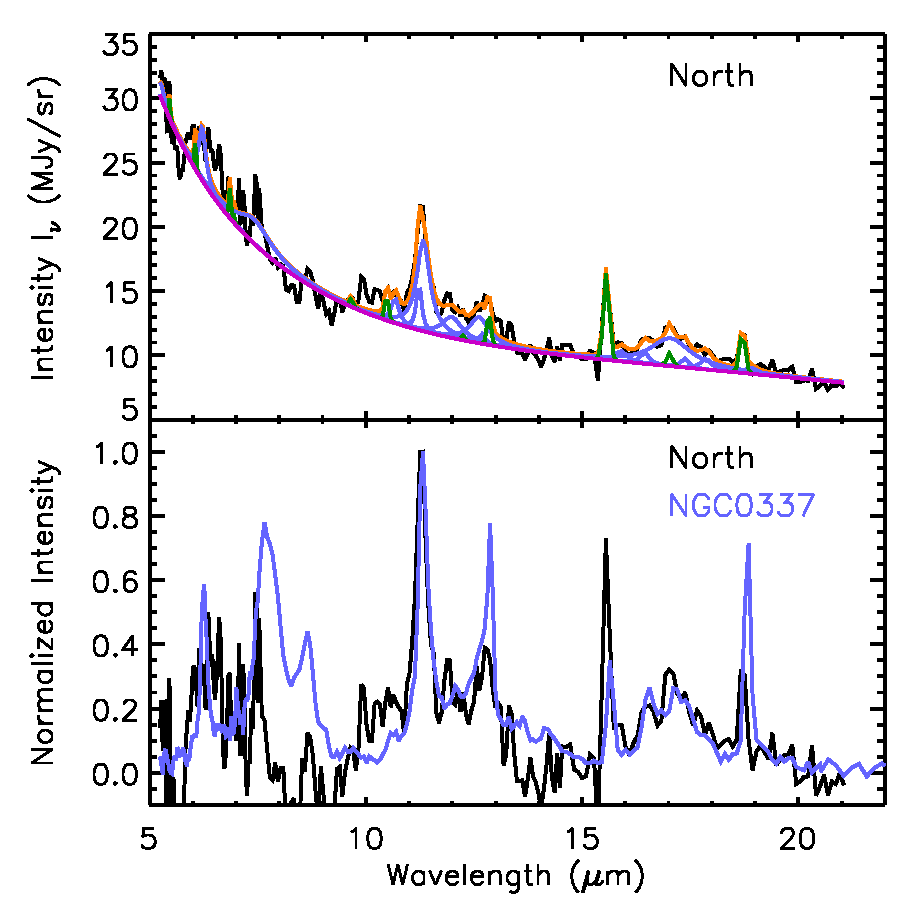
\includegraphics[width = 8 cm]{./fig11.eps}
\caption{Top: PAHFIT result for the extracted spectrum from the north region of the M31 nucleus: fit (orange), continuum (magenta), individual dust components (blue), individual fine-structure lines and H$_2$ lines (green). Bottom: Continuum subtracted spectrum of the north region compared with that of the HII-type galaxy NGC0337 \citep{Smith:2007lr}, normalized to the peak intensity of the  11.2~$\mu$m PAH emission. PAH emission is clearly present longward of~10 $\mu$m. }
\label{fig:nuc_pahfit}
\end{figure}

\begin{figure}
\centering
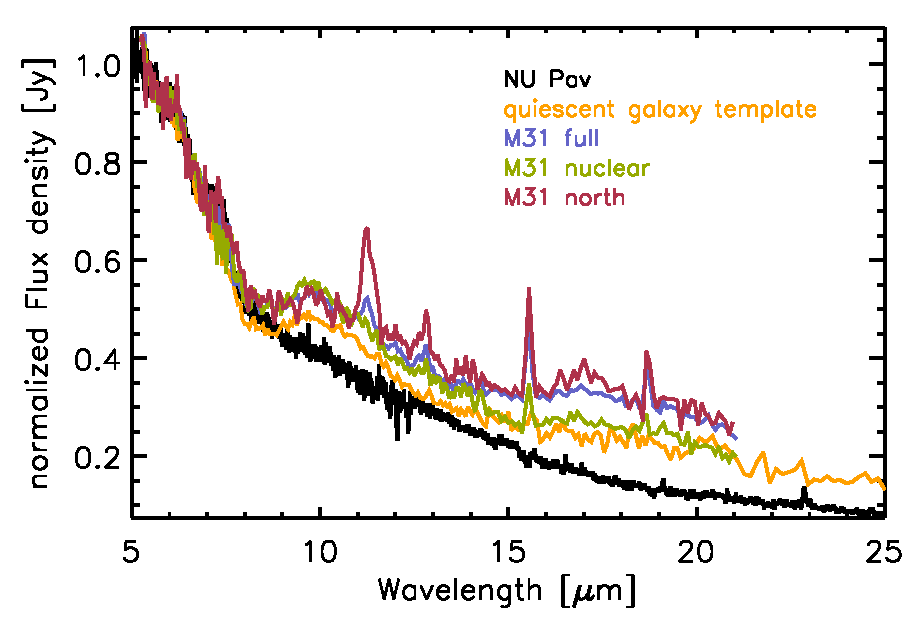
\includegraphics[width = 8 cm]{./fig12.eps}
\caption{Top: Mid-infrared spectrum from the centre region of the M31 nucleus (black) with continuum (magenta). Middle:  Mid-infrared spectrum of the nucleus of M81 \citep[13\arcsec$\times$13\arcsec aperture][black]{Smith2010} with continuum (magenta). Bottom: Normalized continuum-subtracted spectra of the M31 and M81 nuclei. For reference, the silicate optical depth profile towards the galactic centre is shown in blue \citep{Chiar2006}.}
\label{fig:nuc_silicates}
\end{figure}


\begin{figure*}
\centering
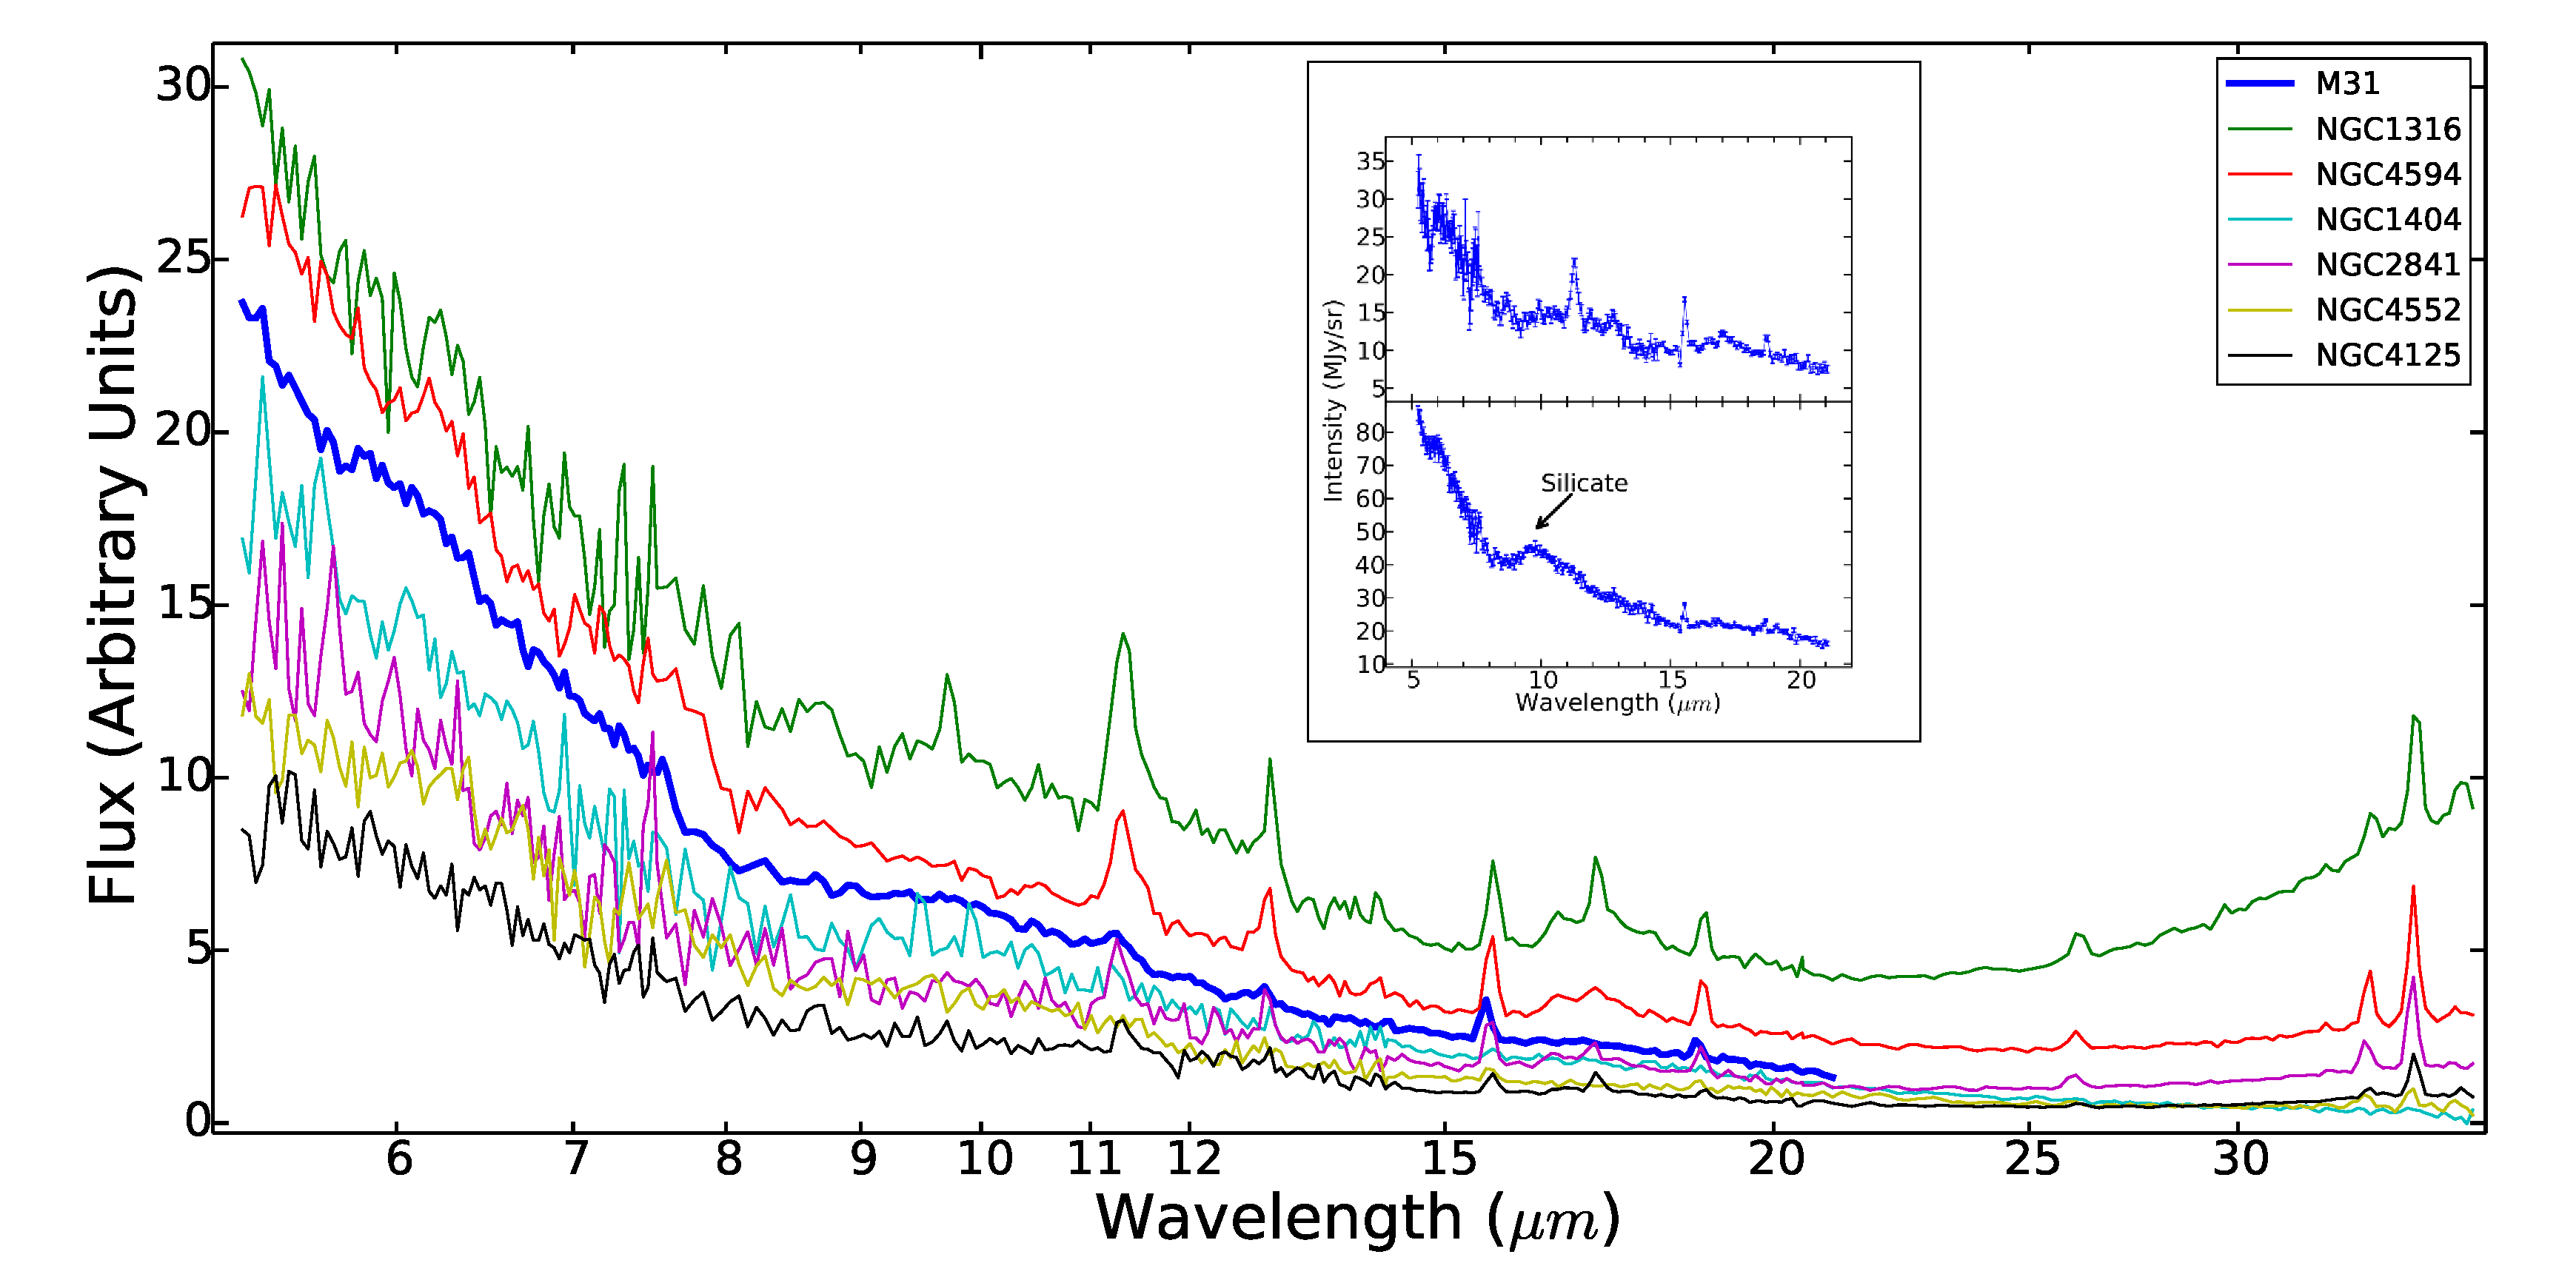
\includegraphics[height = 8 cm]{./fig13.eps}
\caption{Mid-infrared spectrum of the nucleus of M31 (blue) over-plotted with spectra extracted close to the nuclei of 6 nearby galaxies which have 
AGN activity \citep{Smith:2007lr}. NGC 4552, NGC 1404 and NGC 4125 are elliptical galaxies and NGC 4594 and NGC 2841 are spiral galaxies. 
NGC 1316 is a lenticular galaxy. The inset shows the spectra extracted from the centre region of the M31 nucleus (bottom) and from the north region (top) 
shown in Figure \ref{nuc11}.}
\label{smithspec}
\end{figure*}

Figure \ref{smithspec} compares the full 30\arcsec $\times$ 50\arcsec\ M31 nuclear spectrum with the spectra extracted from the smaller regions in the centre and the North (inset, top and bottom). Also shown are nuclear spectra
from six SINGS galaxies with similar spectral shapes \citep{Smith:2007lr}.% 
\footnote{The IRS spectra for the SINGS galaxies were extracted over areas ranging from 2 to 8 kpc$^2$, whereas the M31
nucleus spectrum covers a much smaller area (0.02~kpc$^2$).}
Some SINGS galaxies share similar PAH feature characteristics to the M31 spectrum and none of them contains obvious silicate emission. Although \citet{Mason2012} reported silicate emission towards NGC4594. 
All of these comparison galaxies have some type of LLAGN.
The SINGS galaxies with similar spectral shapes include  three elliptical galaxies, two spirals, and a lenticular; there is some disagreement over the
exact nuclear spectral types of these six galaxies \citep{kennicutt03,Smith:2007lr, moustakas2010}.  All are classified as some form of LLAGN
such as Seyfert or LINER \citep[luminous AGNs were intentionally omitted from the SINGS sample;][]{kennicutt03}, although they are
by no means the only LLAGNs in the SINGS sample.
Published estimates of the black hole masses for these galaxies range from $1.5-5.5\times10^{8}$~M$_{\sun}$
\citep[for NGC~1316 and NGC~4595, respectively]{nowak08, kormendy88}, or about $1-4\times$ that of M31.
M81 is classified as a LINER, with a black hole mass of $7\times10^7$~M$_{\sun}$ \citep{devereux03}.
\citet{Li09} concluded that the central black hole in M31 (M31*) is currently inactive, with direct observational signatures seen only
at radio and X--ray wavelengths, so finding additional signatures in the mid-infrared is of great interest.
To our knowledge, no such signatures have been reported; broadband mid-infrared imaging of the central 
regions of M31 \citep{davidge06,Barmby2006lr} did not identify unambiguous nuclear emission. The bluest
part of the spectrum in Figure~\ref{smithspec} is dominated by the continuum, in agreement with the
expectation that stellar light dominates the nucleus at these wavelengths.


Could radiation from M31* be responsible for the suppression of the  6--8~$\mu$m PAH features compared
to the 11.3~$\mu$m feature?
As discussed by  \citet{Smith:2007lr} and \citet{Smith2010}, inferring such a suppression must be done with caution, 
because the 6--8~$\mu$m features are more susceptible to dilution by the stellar continuum. 
Several connections between PAH suppression and the presence of an AGN are possible, including destruction of small PAH molecules by a hard radiation field, modification of the structure of the PAH molecules, or weak ultraviolet continuum from low star formation rates 
leading to decreased PAH excitation \citep{Smith:2007lr, Diamond2010}.  In the latter case, the AGN is not the cause of the suppressed  6--8~$\mu$m features but rather is only detectable when the nuclear star formation rate is low.
Previous work has found low rates of star formation in the centre of M31: although \citet{Melchior2013} found a significant 
amount of cold gas in the centre of the galaxy, this gas does not appear to be associated with current star formation \citep[see also][]{Li09}.
In modelling the far-infrared spectral energy distribution, \cite{Groves2012} found that  
the old stellar population in the M31 bulge is sufficient to heat the observed dust; no young stellar population is needed. We conclude that PAH feature ratios cannot provide direct evidence for radiation from M31*.


Detection of silicate emission in the M31 nuclear spectrum is another possible indicator of nuclear accretion.
Silicate emission is not very common in integrated spectra of galaxies \citep{Spoon2007} but is seen in luminous 
quasar spectra \citep[e.g.][]{Hill14} and, as mentioned above, in the spectrum of the M81 nucleus. 
In the unified model of AGNs, an obscuring torus viewed face-on would be expected to show silicate emission
\citep{AGNtypes1995, AGNref}; however such a view would also be expected to show forbidden atomic lines such as [Ne~{\sc v}] and [S~{\sc iv}],
not seen in the M31 spectrum. Alternatively, \citet{Mason2012} explained that low-luminosity AGNs cannot 
host a Seyfert-like obscuring torus because of their optically thin dust and low dust-to-gas ratio, but can show
silicate emission that originates in the optically thin hot dust around the central engine.  The first detection of such silicate emission was 
reported by \citet{Sturm2005} from the low-ionization nuclear emission-line region (LINER) galaxy NGC~3998, and 
\citet{Mason2012}  observed that  9.7~$\mu$m silicate emission is present in many LLAGNs. 
To quantify the magnitude of the silicate emission in mid-infrared spectra, \citet{Smith2010} defined
the linear slope parameter $\gamma810 =[F_{\nu}(10\mu{\rm m}) -F_{\nu}(8\mu{\rm m})]/2F_{\nu}(9\mu{\rm m})$,
with positive values signifying silicate emission and negative values absorption. They found the M81 nucleus to have
$\gamma810=0.37\pm0.04$. For the M31 centre (9\arcsec $\times$ 9\arcsec) spectrum, we computed  $\gamma810 =0.01\pm 0.03$,
indicative of neither absorption nor emission. However, for the continuum-subtracted spectrum, we measured   $\gamma810 =1.6\pm 0.4$. This combined with the similar characteristics of the silicate profile in M31 and M81, gives a much stronger indication that silicate emission is detected from M31*.

